\section{Auswertung}
\label{sec:Auswertung}

% % Examples
% \begin{equation}
%   U(t) = a \sin(b t + c) + d
% \end{equation}
%
% \begin{align}
%   a &= \input{build/a.tex} \\
%   b &= \input{build/b.tex} \\
%   c &= \input{build/c.tex} \\
%   d &= \input{build/d.tex} .
% \end{align}
% Die Messdaten und das Ergebnis des Fits sind in Abbildung~\ref{fig:plot} geplottet.
%
% %Tabelle mit Messdaten
% \begin{table}
%   \centering
%   \caption{Messdaten.}
%   \label{tab:data}
%   \sisetup{parse-numbers=false}
%   \begin{tabular}{
% % format 1.3 bedeutet eine Stelle vorm Komma, 3 danach
%     S[table-format=1.3]
%     S[table-format=-1.2]
%     @{${}\pm{}$}
%     S[table-format=1.2]
%     @{\hspace*{3em}\hspace*{\tabcolsep}}
%     S[table-format=1.3]
%     S[table-format=-1.2]
%     @{${}\pm{}$}
%     S[table-format=1.2]
%   }
%     \toprule
%     {$t \:/\: \si{\milli\second}$} & \multicolumn{2}{c}{$U \:/\: \si{\kilo\volt}$\hspace*{3em}} &
%     {$t \:/\: \si{\milli\second}$} & \multicolumn{2}{c}{$U \:/\: \si{\kilo\volt}$} \\
%     \midrule
%     \input{build/table.tex}
%     \bottomrule
%   \end{tabular}
% \end{table}
%
% % Standard Plot
% \begin{figure}
%   \centering
%   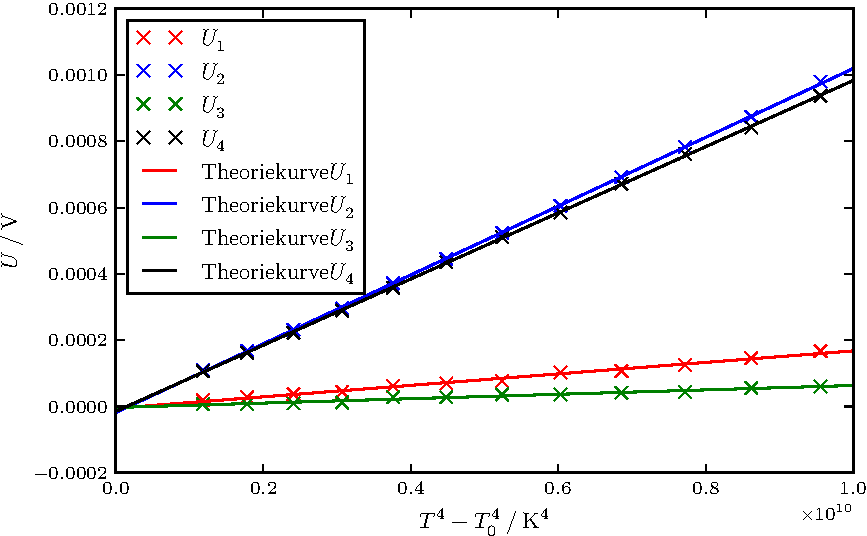
\includegraphics{build/plot.pdf}
%   \caption{Messdaten und Fitergebnis.}
%   \label{fig:plot}
% \end{figure}
%
% 2x2 Plot
% \begin{figure*}
%     \centering
%     \begin{subfigure}[b]{0.475\textwidth}
%         \centering
%         \includegraphics[width=\textwidth]{Abbildungen/Schaltung1.pdf}
%         \caption[]%
%         {{\small Schaltung 1.}}
%         \label{fig:Schaltung1}
%     \end{subfigure}
%     \hfill
%     \begin{subfigure}[b]{0.475\textwidth}
%         \centering
%         \includegraphics[width=\textwidth]{Abbildungen/Schaltung2.pdf}
%         \caption[]%
%         {{\small Schaltung 2.}}
%         \label{fig:Schaltung2}
%     \end{subfigure}
%     \vskip\baselineskip
%     \begin{subfigure}[b]{0.475\textwidth}
%         \centering
%         \includegraphics[width=\textwidth]{Abbildungen/Schaltung4.pdf}    % Zahlen vertauscht ... -.-
%         \caption[]%
%         {{\small Schaltung 3.}}
%         \label{fig:Schaltung3}
%     \end{subfigure}
%     \quad
%     \begin{subfigure}[b]{0.475\textwidth}
%         \centering
%         \includegraphics[width=\textwidth]{Abbildungen/Schaltung3.pdf}
%         \caption[]%
%         {{\small Schaltung 4.}}
%         \label{fig:Schaltung4}
%     \end{subfigure}
%     \caption[]
%     {Ersatzschaltbilder der verschiedenen Teilaufgaben.}
%     \label{fig:Schaltungen}
% \end{figure*}

\subsection{Überprüfung der Bragg Bedingung}
Um die ausreichende Kalibrierung des Gerätes festzustellen, wird zunächst die in der Durchführung beschriebene Kontrolle der Bragg-Bedingung durchgeführt.
Die Ergebnisse der Messung sind in Abbildung \ref{fig:plot1} dargestellt.
\begin{figure}
  \centering
  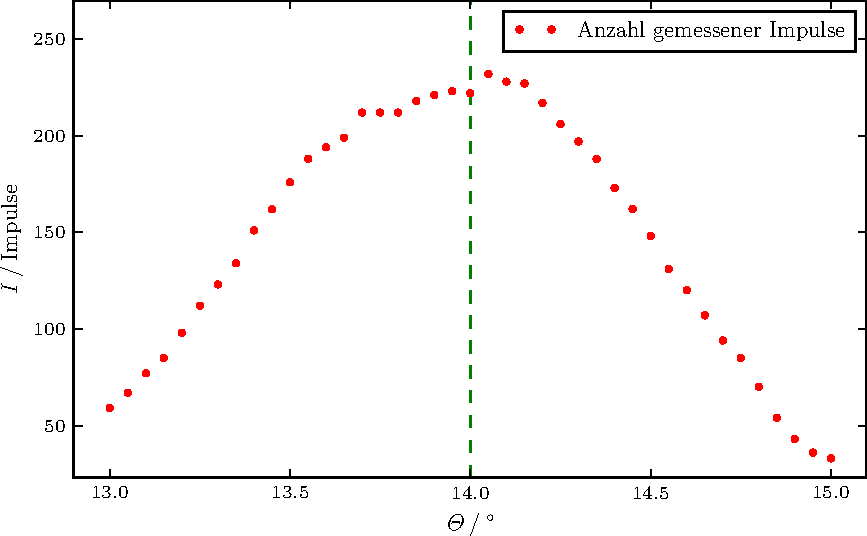
\includegraphics{build/plot_1.pdf}
  \caption{Messwerte zur Prüfung der Bragg Bedingung.}
  \label{fig:plot1}
\end{figure}
Der Peak ist in etwa gleichmäßig um den erwarteten Winkel von $\Theta = \SI{14}{\degree}$ zentriert.

\subsection{Emissionsspektrum der Kupfer-Röntgen-Röhre}
Wie in der Durchführung beschrieben wird das Emissionsspektrum der Röntgenröhre durchlaufen.
Das gemessene Röntgenspektrum ist in Abbildung \ref{fig:plot2} angegeben.
\begin{figure}
  \centering
  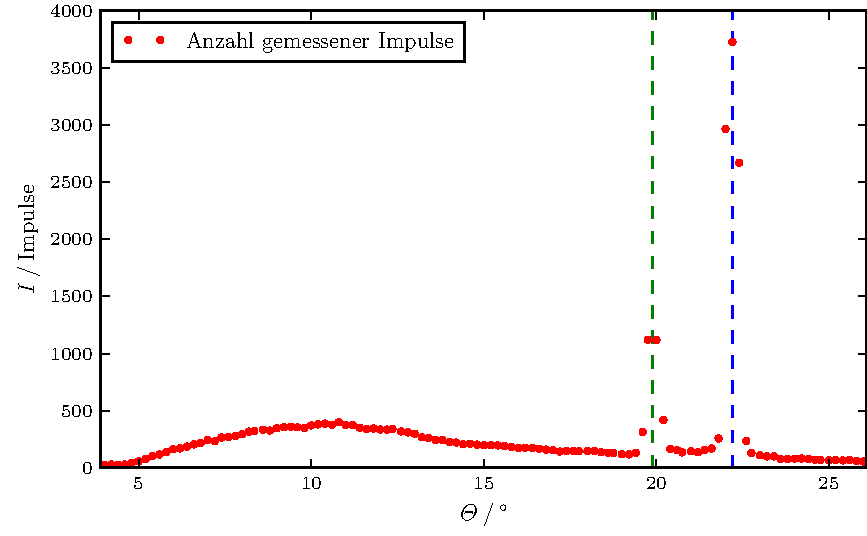
\includegraphics{build/plot_2.pdf}
  \caption{Emissionsspektrum der Kupfer-Anode.}
  \label{fig:plot2}
\end{figure}
Als Peaks des Spektrums lassen sich die Winkel
\begin{align*}
   \Theta_{K_\alpha} &= \SI{22.2}{\degree}
 \\
   \Theta_{K_\beta} &= \SI{19.9}{\degree}
 \\
\end{align*}
ablesen und als die jeweiligen Linien identifizieren.
Nach Formel \eqref{eqn:bragg} bestimmen sich die Energien zu
\begin{align*}
  E_{K_\alpha} &= \SI{8.15}{\kilo\electronvolt}
 \\
  E_{K_\beta} &= \SI{9.05}{\kilo\electronvolt}
. \\
\end{align*}
Zur Untersuchung des Bremsbergs bzw. zur Bestimmung der maximalen Energie des Bremsspektrums wird das Emissionsspektrum für den Grenzbereich ein weiteres mal mit einer höheren Auflösung gemessen.
Das Ergebnis ist in Abbildung \ref{fig:plot3} graphisch dargestellt.
\begin{figure}
  \centering
  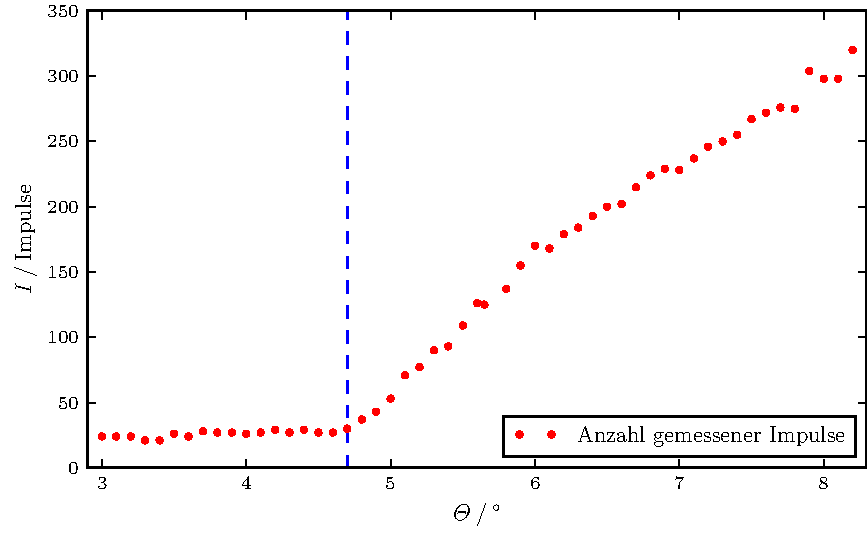
\includegraphics{build/plot_3.pdf}
  \caption{Emissionsspektrum der Kupfer-Anode (Maximale Kante).}
  \label{fig:plot3}
\end{figure}
Der auftretende Grenzwinkel beträgt
\begin{align*}
  \Theta_{\text{grenz}} = \SI{4.7}{\degree}
 \\
\end{align*}
was sich mit Hilfe von Formel \eqref{eqn:bragg} zu einer minimalen Wellenlänge von
\begin{align*}
  \lambda_{\text{min}} = \SI{33.0}{\pico\metre}

\end{align*}
beziehungsweise einer maximalen Energie von
\begin{align*}
  E_{\text{max}} = \SI{37.6}{\kilo\electronvolt}

\end{align*}
umrechnen lässt.\\
Aus den Energien $E_{K_\alpha}$ und $E_{K_\beta}$ lassen sich aus Formel \eqref{eqn:sigma} die Abschirmkonstanten $\sigma_K$ bestimmen.
